\chapter{Introduction to Deep Learning}

\section{Motivation}
\paragraph{Example: is AI like Alchemy?}

A core of deep learning is to optimize a loss function with respect to a collection of model parameters. In NIPS 2017 talk, Rahimi gives a typical example for choosing parameters for a 2-layer neural network.
\begin{figure}[H]
\centering
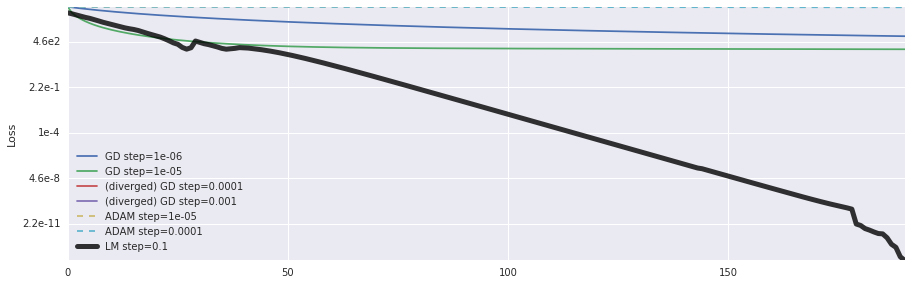
\includegraphics[width=0.8\textwidth]{First_lecture/p_1.jpg}
\caption{Numerical Results for solving $\min_{W_1,W_2}\hat{\mathbb{E}}\|W_1W_2x-Ax\|^2$}
\end{figure}
The gradient descent for solving this problem gets stuck at the objective value~(error) around $400$. In particular,
\begin{itemize}
\item
It does not converge to a stationary point
\item
This phenomenon is not due to the statistical noise floor of the dataset. Computing the expectation of the loss and directly minimize it leads to the same result.
\end{itemize}
Rahimi reveals that gradient descent cannot usually solve a $2$-layer linear network. However, we expect it to solve a $1000$-layer neural-net with $1$ million data.
It seems we don't understand neural-net optimization at all. 

LeCun has a different pespective. He thinks that having theory for deep learning is important, but another goal is to invent new methods, new tricks, etc. Perhaps we don't have or don't need theory for neural networks.


\paragraph{Comment from Ruoyu Sun}
\begin{enumerate}
\item
Do we need to study deep learning?

For application researchers, there is no doubt. For applications, Neural-nets (not necessarily current deep learning) will probably become fundamental tool in many fields.
For theoretical researchers such as optimizers, mathematicians, statisticians, this is still a big question. 
Deep learning is possible to become a theoretical field.
\item
Do we need theory for deep learning?

Yes, since we need to \emph{udnerstand} why deep learning works. There are tons of hard deep learning problems, and we need to solve them. Moreover, theory can help deep learning work for other fields such as reinforcement learning, physics, biology, etc.
\item
This course tries to offer answers to these questions, but it cannot answer them completely, not even a $20\%$ answer. We will analysis deep learning from the perspective of optimization, and understand why some heuristics can help.
\end{enumerate}

\section{Outline}
\paragraph{Pre-requisite}
\begin{itemize}
\item
Pre-requisites: Calculus, Linear Algebra, Probability, Optimization, and Basics of Deep Learning.
\item
Related Subjects (helpful but not required): Basic knowledge from compute vision and NLP, the trend of Deep Learning and Artificial Intelligence.
\end{itemize}
%\paragraph{Grading Policy}
%3-4 assignements and a simple course project.
\paragraph{Course Objective and Audience}
This course will talk about optimization theory of deep learning. This is not intended for practitioners with little interest in theory, and want to know how to tune parameters. 
Intended audience:
\begin{itemize}
\item
Theorists (e.g., optimizers, machine learners, statisticians, mathematicians,
theoretical computer scientists) who want to work on or
interested in theory of deep learning;
\item
Practitioners interested in theory;
\item
Those who curious about frontiers of optimization in deep learning.
\end{itemize}
Also note that the theory discussed in this course does not necessarily solve real problems in deep learning, but it offers the logic of thinking that is the most helpful.

\section{Neural Network Basis}\label{sec:1:3}
Firstly, we will give mathematical descriptions of fully-connected neural networks. The Figure~(\ref{fig:1:2}) gives a demostration of $3$-layer fully-connected neural network. Neural networks give a function $f:\mathbb{R}^{d_x}\to\mathbb{R}^{d_y}$ parameterized with $\theta\in\mathbb{R}^{d_\theta}$:
\begin{itemize}
\item
Input: $x\in \mathbb{R}^{d_x}$;
\item
Output: $y\in \mathbb{R}^{d_y}$;
\item
A $L$-layer fully connected neural network consists of $L-1$ hidden layers.
\item
The values of the next hidden layer are a linear transformation of previous values, and then followed by a non-linear function:
\[
\begin{array}{ll}
\mbox{pre-activiation}:&h^{\ell}=W^{\ell}z^{\ell-1},\quad\ell=1,\dots,L\\
\mbox{post-activation}:&z^{\ell}=\phi(h^{\ell}),\quad\ell=1,\dots,L
\end{array}
\]
Here $W^{\ell}\in\mathbb{R}^{d_{\ell}\times d_{\ell-1}}$ denotes the weight matrix, and $\phi$ denotes the nonlinear function.
\end{itemize}
Using the notions above, the function $f_\theta$ can be written as
\begin{equation}
f_{\theta}(x) = W^{L}\phi(W^{L-1}\phi(\cdots\phi(Wx)))
\end{equation}
\begin{figure}
\centering
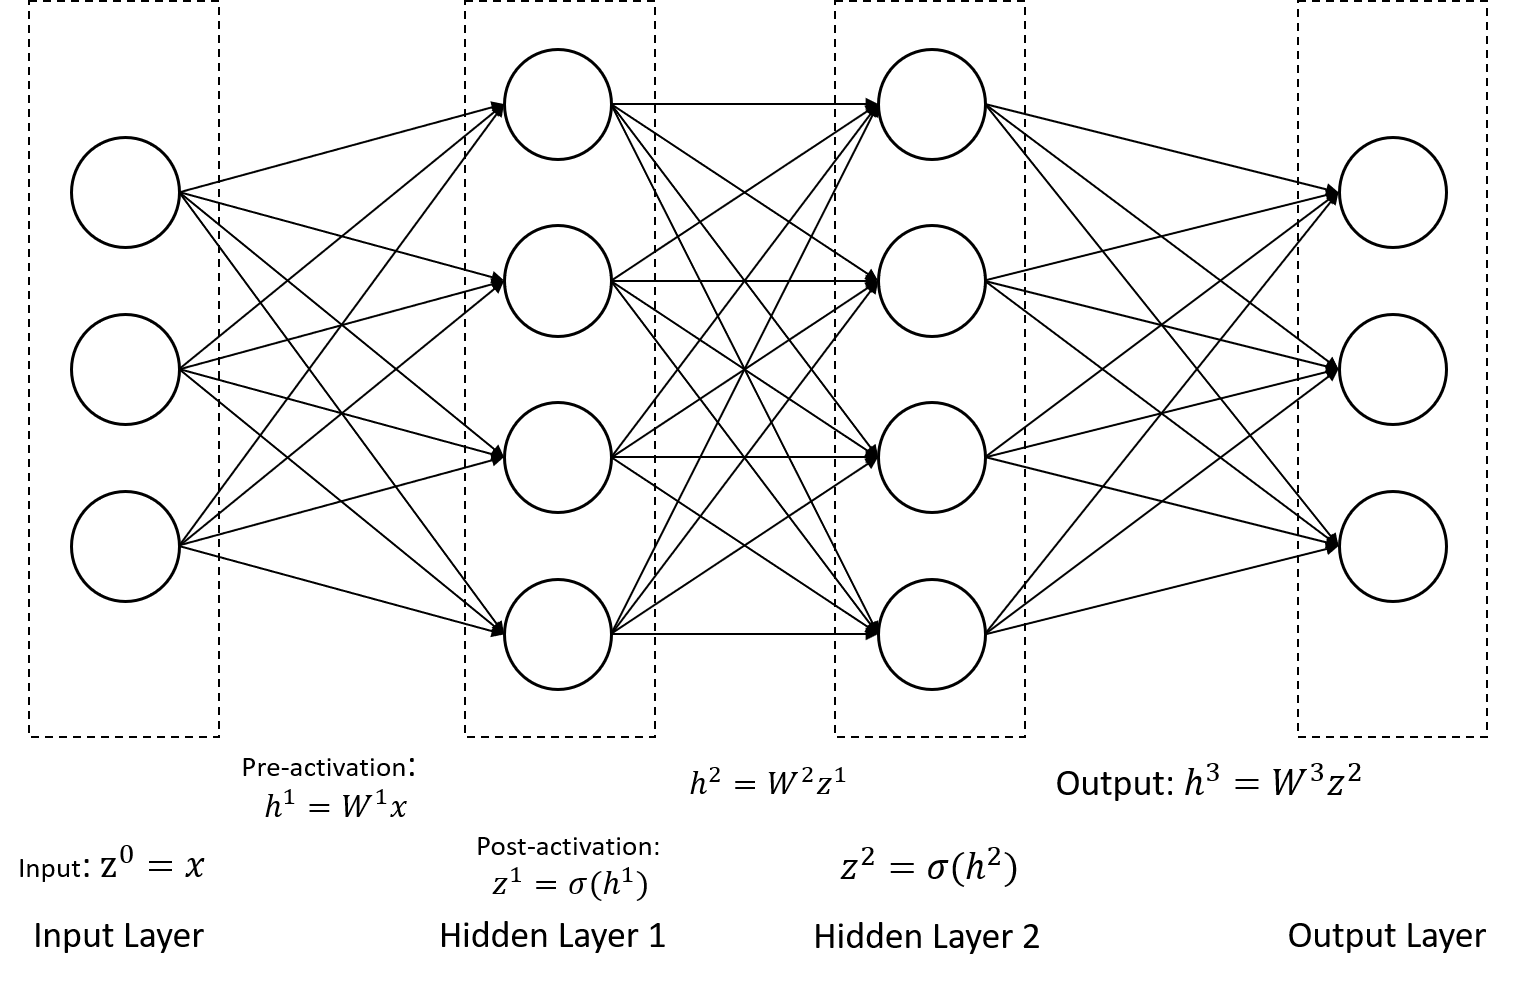
\includegraphics[width=0.9\textwidth]{First_lecture/p_2}
\caption{Example of a $3$-layer fully-connected neural network.}
\label{fig:1:2}
\end{figure}
\begin{remark}
The bias of the neural network is skipped. In general, it should be $z^{\ell}=\phi(W^{\ell}z^{\ell-1}+b^{\ell})$.
\end{remark}
\begin{remark}
There are other kinds of neural network, such as CNN, RNN, and ResNet.
\end{remark}
\paragraph{Why $\&$ When $\&$ How do we need neural-nets?}
Consider the image classificaiton scenario. 
Imagine there is an orcle telling you the label of the input image, say $f^*$.
The motivation for using deep learning is that it can approximate such a function very well.
The classical way for applying deep learning is the supervised learning:
\begin{quotation}
Given data $(x_i,y_i)$ for $i=1,\dots,n$, we need to find a model $f_\theta$ from a set of model candiates $\mathcal{F}$ such that $f_\theta(x_i)\approx y_i$, $i=1,\dots,n$.
\end{quotation}
This problem is often formulated as a finite-sum optimization problem:
\[
\min_\theta\frac{1}{n}\sum_{i=1}^n\ell(f_{\theta}(x_i),y_i),
\]
where $\ell(\cdot,\cdot)$ denotes the loss function.
\begin{enumerate}
\item
When the representation model $f_\theta(x)=Wx$, and the loss is quadratic, the problems becomes a least-square linear regression problem
\item
 When the representation is a $2$-layer neural network, say $f_\theta(x)=W^2W^1x$ and the loss is quadratic, the problem becomes
 \[
 \min_{W^2,W^1}\sum_{i}\|y_i-W^2W^1x_i\|^2 = \|Y-W^2W^1X\|_F^2
 \]
 When $X=I$, this problem reduces to the matrix factorization problem:
 \begin{equation}
\min_{U,V}\|Y-UV\|_F^2
\end{equation}
For matrix $Y\in \mathbb{R}^{m\times n}$ and decision variables $U\in\mathbb{R}^{m\times p},V\in\mathbb{R}^{p\times n}$, if $p<\rank(Y)$, then the optimal solution
\[
U^*=\begin{pmatrix}
\sqrt{\sigma_1}u_1&\cdots&\sqrt{\sigma_p}u_p
\end{pmatrix},\quad
V^*=\begin{pmatrix}
\sqrt{\sigma_1}v_1&\cdots&\sqrt{\sigma_p}v_p
\end{pmatrix}\trans
\]
where $\{u_i,v_i,\sigma_i\}_{1:p}$ are from the first $p$ terms of the SVD decomposition of $Y$.

\end{enumerate}

\section{Gradient Explosion/Vanishing}\label{sec:1:4}
Consider minimizing a quadratic loss for multi-layer neural network with scalar input:
\[
\min_{w_1,\dots,w_L}F(w)\triangleq\frac{1}{2}(1-w_1\cdots w_L)^2
\]
\paragraph{Solving by Classical Gradient Descent}
If applying gradient descent, the step size should be bounded by 1 over the Lipschitz constant $\beta$ of the objective function. 
Here we compute this constant:
\begin{align*}
\frac{\partial F}{\partial w_1}&=-(1-w_1\cdots w_L)w_2\cdots w_L\\
\frac{\partial^2 F}{\partial w_1^2}&=(w_2\cdots w_L)^2
\end{align*}
Note that $L\approx\lambda_{\max}(\nabla^2_{w}F)$. Here we simply use $\frac{\partial^2 F}{\partial w_1^2}$ to loosely study how large~(small)$\beta$ is.
\begin{itemize}
\item
When $w_2=\cdots=w_L=2$, then $\beta=2^{\mathcal{O}(L)}$
\item
When $w_2=\cdots=w_L=\frac{1}{2}$, then $\beta=2^{-\mathcal{O}(L)}$
\end{itemize}
Take $L=100$ as an example. For the first initialization, the step-size is too big; for the second initialization, the step size is too small.
This issue is called \emph{Lipschitz constant explosion/vanishing}.






%
%\section{Building (distributed, learned) first order methods from monotone operators}
%
%\begin{definition}
%Pick $x\ne y$ and $u\in Ax$, $v\in Ay$. Plot a complex $z=re^{\phi i}$ such that
%\[
%r = \frac{\|u-v\|}{\|x-y\|},\quad \phi:=\text{angle}(u-v,x-y)
%\]
%In general, $z$ depends on $(x,u),(y,v)$. Therefore,
%\[
%\mathcal{G}(A)=\{z:x\ne y, u\in Ax,v\in Ay\}\cup\{\{\infty\}\text{ if $A$ is multi-valued}\}
%\]
%It's called the scaled relative graph~(SRG).
%\end{definition}
%\begin{proposition}\label{pro:1:1}
%If the operator $\mathcal{A}\subseteq\mathcal{B}$, then $\mathcal{G}(A)\subseteq\mathcal{G}(B)$ always holds.
%\end{proposition}
%
%\begin{example}
%Projection to any line, subdifferential of $\ell_2$ norm.
%\end{example}
%\begin{definition}
%Given a class of operator $\mathcal{A}$, $\mathcal{G}(\mathcal{A})=\cup_{A\in \mathcal{A}}A$
%\end{definition}
%\begin{example}
%From optimization.
%\end{example}
%\begin{definition}[Monotone Operators]
%s
%\end{definition}
%\begin{example}
%Monotone Operators for linear convergence
%\end{example}
%\begin{example}
%Monotone Operators for sub-linear convergence
%\end{example}
%
%Question: when does the converse of (\ref{pro:1:1}) holds?
%We say if it is true, $\mathcal{B}$ is SRG-full.
%\begin{example}
%Many oerator classes are SRG-full classes.
%\end{example}
%
%\begin{definition}
%Forward operator of $A$:
%\[
%F_{\alpha A}=I-\alpha A
%\]
%\end{definition}
%SRG is under sclaing and translation:
%\[
%\mathcal{G}(\alpha I+\beta\mathcal{A})=\alpha +\beta\mathcal{G}(\mathcal{A}),\quad\alpha,\beta\in\mathbb{R}
%\]
%\begin{example}
%Classic optimization proposition by graphic proof.
%
%Counter-example. If graph not contain
%\end{example}
%\begin{definition}
%Inverse operator of $A$, say $A^{-1}$:
%\[
%A^{-1}y = \{x:y\in Ax\}
%\]
%Backward operator of $A$:
%\[
%J_{\alpha A}=(I+\alpha A)^{-1}
%\]
%\end{definition}
%\begin{definition}[Splitting]
%
%\end{definition}
%\begin{proposition}
%If $\mathcal{A},\mathcal{B}$ are SRG-full, then 
%\[
%\mathcal{G}(\mathcal{AB})\supseteq\mathcal{G}(\mathcal{A})\mathcal{G}(\mathcal{B})
%\]
%\end{proposition}
%
%\begin{example}[Pnp Operator]
%
%\end{example}
%
%\begin{example}[ADMM]
%
%\end{example}
%\section{Mathematics of Deep Learning}
%\paragraph{Motivation}
%\begin{itemize}
%\item
%Extract math or theory of DL
%\item
%Theory: model that explain and predict
%\item
%Math: framework + understanidng, help design
%\end{itemize}
%
%\paragraph{Supervised learning: Formulation}
%
%\begin{itemize}
%\item
%Representation
%\item
%Optimization
%\item
%Generalization
%\end{itemize}
%\paragraph{Why DL success?}
%Data, algorithm, Computation power.
%
%\paragraph{Representation Theory of DL}
%\emph{Deep} neural-nets are much more \emph{efficient} in representing a funciton than \emph{shallow} neural-nets.
%
%Neural-net:
%\begin{itemize}
%\item
%1-hidden-layer net: $\hat{y} = v\trans\phi(Wh)$
%\[
%\mathcal{F}=\{f_\theta\mid f_\theta(x) = W^2\phi(W^1x)\}
%\]
%\item
%2-hidden-layer nets: $\hat{y} = W^3\phi(W^2\phi(W^1h))$
%\end{itemize}
%
%
%\begin{itemize}
%\item
%Deep-nets are more efficient approximators
%\item
%Example: 
%\item
%New research: Limitations
%\end{itemize}
%\paragraph{Optimization Theory of DL}
%\begin{itemize}
%\item
%Level 1: Decomposition, i.e., test error = traning error + generalization error
%\item
%Level 2: Training error = Representation error + optimization error
%\item
%Level 3:
%\end{itemize}
%Topic:
%\begin{itemize}
%\item
%How to make the algorithm converge? 
%\item
%Landscape of objective function.
%\end{itemize}
%
%\paragraph{Deep NN traning is difficult}
%
%
%
%\paragraph{Landscape}
%
%\section{Historical Perspective on the ADMM}
%Starting point: augmented Lagrangian method introduced in 1960s by M. Hestenes and M.Powell. 
%\[\begin{array}{ll}
%\min&J(y)=\frac{1}{2}y\trans Ay - b\trans y\\
%&Bx=c
%\end{array}
%\]
%This is solved by KKT condition:
%\[
%\mathcal{L}(y)
%\]
%
%\section{Recent Development of ADMM}
%\subsection{Two-Block ADMM}
%\[
%\begin{array}{ll}
%\min&\theta(x):=\theta_1(x_1)+\theta_2(x_2)\\
%&A_1x_1+A_2x_2=b, x_i\in\Omega_i
%\end{array}
%\]
%Classic ADMM. 
%Application: image and signal processing, compressive sensing [Yin's work].
%
%Convergence established for block two.
%
%\paragraph{Convergence Rate}
%\begin{itemize}
%\item
%The measure of optimality: $(x^*,\lambda^*)$ should be saddle point
%\item
%General results
%\item
%Specific assumptions.
%\end{itemize}
%
%Make the ADMM fast:
%\begin{itemize}
%\item
%update step size
%\item
%Do the extrapolation to $(x,\lambda)$
%\end{itemize}
%
%
%\subsection{Multi-Block ADMM}
%
%Multi-block ADMM can diverge. How to make it converge:
%\begin{itemize}
%\item
%If without additonal steps,
%\begin{itemize}
%\item
%assume additonal assumptions:
%\begin{itemize}
%\item
%strongly convexity is not enough
%\end{itemize}
%\item
%restrict the parameter $\beta$ and $\beta$
%\end{itemize}
%\item
%with additional steps: handle the unfairness of the update of block variables. (how to handle.)
%\begin{itemize}
%\item
%Prediction-correction type methods
%\item
%Gaussian Back substitution
%\item
%Randomly Permuted ADMM (assumptions?)
%\end{itemize}
%Work for general convex separable problems
%\end{itemize}
%How when subproblem has non-unique solution?
%\emph{uniqueness of solutions for subproblems}
%
%
%
%
%\subsection{Non-convex ADMM}
%
%Key idea: sufficient decrease of a merit function and use the structure (K-L inequality with exponent $\alpha$)
%\[
%\text{dist}(0,\partial f(x))\ge (f(x) - f(\bar{x}))^{\alpha}
%\]
%\section{Meta-Learning}
%For unconstrained optimization $\min F(x)$, write $x^* = f(F)$. 
%
%Solving linear systems by meta-learning:
%\begin{itemize}
%\item
%Sample a set of problem instances $\{(A_i,b_i)\}_{i=1:N}$
%\item
%Paraneterize the solution $x=f(A,b)$ by a deep neural network $x=f_\theta(A,b)$
%\item
%Find the optimal $\theta^*$ by solving the non-linear least squares
%\item
%Evaluate the performance of solver $f_{\theta^*}(A,b)$ over test problems drawn from the same distribution
%\end{itemize}
%This is sample inefficient. The idea is to introduce bias, i.e., decompsoing the solution process into stages, .e.g.,
%\[
%x=f(A,b)=f_1(A,f_2(f_3(A,b),A,b),A,b)
%\]
%just learn one component function.
%
%
%\section{Large-Scale LP Decoding}
%
%
%\section{Priml-Dual Dynamical Approach}
%\[
%\min_{x\in\mathcal{H}}h(x)
%\implies
%\left\{
%\begin{aligned}
%\dot{x}(t)&=-\nabla h(x(t))\\
%x(0)&=x^0
%\end{aligned}
%\right.
%\]
%or $f$ is lower semi-continuous:
%\[
%\left\{
%\begin{aligned}
%\dot{x}(t)&\in \partial f(x(t))\\
%x(0)&=x^0
%\end{aligned}
%\right.
%\]
%Explicit time discretization leads to the subgradient method;
%Implicit time discretization leads to the proximal method
%\[
%\min_{x\in C}h(x)
%\implies
%\left\{
%\begin{aligned}
%\dot{x}(t)+x(t)&=\text{prox}_{C}(x(t) - \gamma \nabla h(x(t)))\\
%x(0)&=x^0
%\end{aligned}
%\right.
%\]
%\[
%\min_{x\in\mathcal{H}}f(x)+h(x)
%\implies
%\left\{
%\begin{aligned}
%\dot{x}(t)+x(t)&=\text{prox}_{\gamma f}(x(t) - \gamma \nabla h(x(t)))\\
%x(0)&=x^0
%\end{aligned}
%\right.
%\]
%
%Time discretiztion of continuous dynamical systems lead usually to different iterative schemes.
%
%Consider the structured convex minimization
%\[
%\min_{x\in\mathcal{H}}f(x)+h(x)+g(Ax)
%\]
%
%\section{Higher Order Tensor Method for Convex Optimization}
%\[
%\min_{x\in\mathbb{R}^n}f(x),
%\]
%where $f$ is $p$-times differentiable.
%\[
%\nabla^pf(x)_{i_1,\dots,i_p}=\frac{\partial^pf}{\partial x_{i_1,\dots,i_p}}(x)
%\]
%The $\nabla ^pf$ is Lipschitz continuous. The norm of $\nabla^pf(x)$ is defined based on directional derivative.
%\[
%\|\nabla^pf(x)\| = \max_{\|h^j\|=1,j=1,\dots,p}\nabla^pf(x)[h^1,\dots,h^p]
%\]
%
%
%\section{Distributed non-convex Optimization}
%
%\[
%\begin{array}{ll}
%\min_{x\in\mathbb{R}^p}&g(y) = \frac{1}{M}\sum_{i=1}^Mf_i(x_i)\\
%\text{s.t. }&Ax=0
%\end{array}
%\]
%\section{Second Order Method}
%\[
%\min_{x}\psi(x) = f(x)+\phi(x)
%\]
%where $f(x)$ is of expectation / finite-sum form.
%
%First order:
%\begin{itemize}
%\item
%easy to implement, converge fast ot a solution
%\item
%slow tail convergence
%\end{itemize}
%
%Proximal Gradient Method
%\[
%x^{k+1} = \arg\min_{x}\inp{\nabla f(x^k)}{x-x^k}+\frac{1}{2t}\|x-x^k\|_2^2+\phi(x)
%\]
%Use Newton method to solve in each iteration. Difficulty: the proximal operator is non-differentiable. However, it is semi-smooth.
%
%Application on Deep RL:
%
%\section{First Order Method}
%\[
%\begin{array}{ll}
%\min_{x\in X}&f(x)\\
%&c_i(x)=0\\
%&g_j(x)\le 0
%\end{array}
%\]
%where $X$ is a simple closed bounded convex set;
%$f$ is smooth and possibly non-convex;
%$c_i$ and $g_j$ are smooth and possibly non-convex functions;
%projection onto the feasible set is expansive.
%
%The goal is to establish complexity results for finding near-KKT points by accessing function value and gradient information.
%\begin{align*}
%\text{dist}(0, \nabla_x(x,y,z)+\mathcal{N}_X(x))&\le \epsilon, z^k\ge 0\\
%\|[c_1,\dots,c_{\ell}(x)]\|+\|[g_1(x),\dots,g_m(x)]\|&\le\epsilon\\
%|z_jg_j(x)|&\le\epsilon,\ \forall j=1,\dots,m
%\end{align*}
%\paragraph{Convex Objective and Convex Constraints}
%Then there exists a KKT point.
%Example: portfolio selection
%
%Introduce slack variables to derive augmented Lagrangian function. Inexact augmented Lagrangian method.
%
%\section{Proximal Point Algorithm}
%Opeator Inclusion Problem: find $w^*\in\mathbb{R}^d$ such that
%\[
%0\in T(w^*),\quad \text{or }w^*\in T^{-1}(0)
%\]
%If $T$ is maximal monotone, then its resolvent operator $J_T=(I+T)^{-1}$ is single-valued and everywhere defined.
%
%Note that $0\in T(w^*)$ iff $w^*=J_{\lambda T}(w^*)$.
%
%The classical method of multipliers or augmented Lagrangian method is a dual application of PPA.
%The DR operator splitting method is also an application of the PPA.
%
%\paragraph{Convergence}
%\begin{itemize}
%\item
%PPA converges globally under mild conditions, enjoys fast local linear/superlinear convergence under regularity conditions.
%\item
%$\mathcal{O}(1/N)$ sublinear convergence rate measured by fixed point residual for PPA and DR.
%\item
%Ergodic $\mathcal{O}(1/N)$ sublinear convergence rate for monotone variational inequality problems.
%\end{itemize}
%
%
%
%
%
%
%
%
%
%
%
%
%
%
%
%
%
%
%
%
%
%
%
%
%
%
%
%
%
%
%
%
%
%
